\chapter{Оршил}
\section{Үндэслэл}
Бакалаврын судалгааны ажлаар инженерчлэлийн чиглэлээр хийж буй энэхүү бүтээл нь програмчлал болон архитектур, зохиомжлолын хүрээнд олон мэдлэг чадвар, судалгааг шаардаж байгаа бөгөөд миний бие Нямдоржийн Энхболд өөрийн сурсан мэдлэгээ өнөөгийн технологиудын судлагаа, практиктай хослуулан энэхүү вебэд суурилсан системийг хийвэл зохино гэж үзэв. 

Монголд ашиглагдаж буй ихэнх програмчлалын бодлого боддог платформ/системүүд нь ихэвчлэн гадных байдаг бөгөөд өөрсдийн үүсгэсэн бодлогын санг оруулж хэрэглэж байгаа билээ. Програмчлалд суралцаж буй сурагч, оюутан залууст эх хэл дээр нь хэлний бэрхшээлээс ангид байдлаар суралцах боломжийг олгох нь сурах процесст эергээр нөлөөлдөг бөгөөд одоогоор Монголд хэрэгжүүлсэн системүүд маш цөөхөн, мөн өөр зорилго агуулсан байдаг.

Алгоритм болон програмчлалын салбарт өөрийн хувь нэмрээ оруулна гэх мотивацын дор энэхүү системийг хэрэгжүүлэх сэдэл төрсөн билээ.

\section{Зорилго}
Уг бүтээл нь цаашаа төсөл байдлаар урт хугацаанд хэрэгжих бөгөөд инженерчлэлийн судалгааны ажлаар MVP(Minimum viable product)-ийг бий болгохыг зорьсон.

"Coldbrains" гэх систем нь хэрэглэгчийн сурсан програмчлалын мэдлэг чадваруудыг бататгах болон үнэлэх зорилготой бөгөөд хэрэглэгч өөрийн түвшинг тодорхойлох, цаашлаад тулгарсан програмчлалын асуудлуудад ямар аргуудыг ашиглах боломжтой байдаг талаарх ойлголтуудыг хуваалцах билээ.

% \section{Үечилсэн төлөвлөгөө}
% \begin{figure}[h]
%   \centering
%   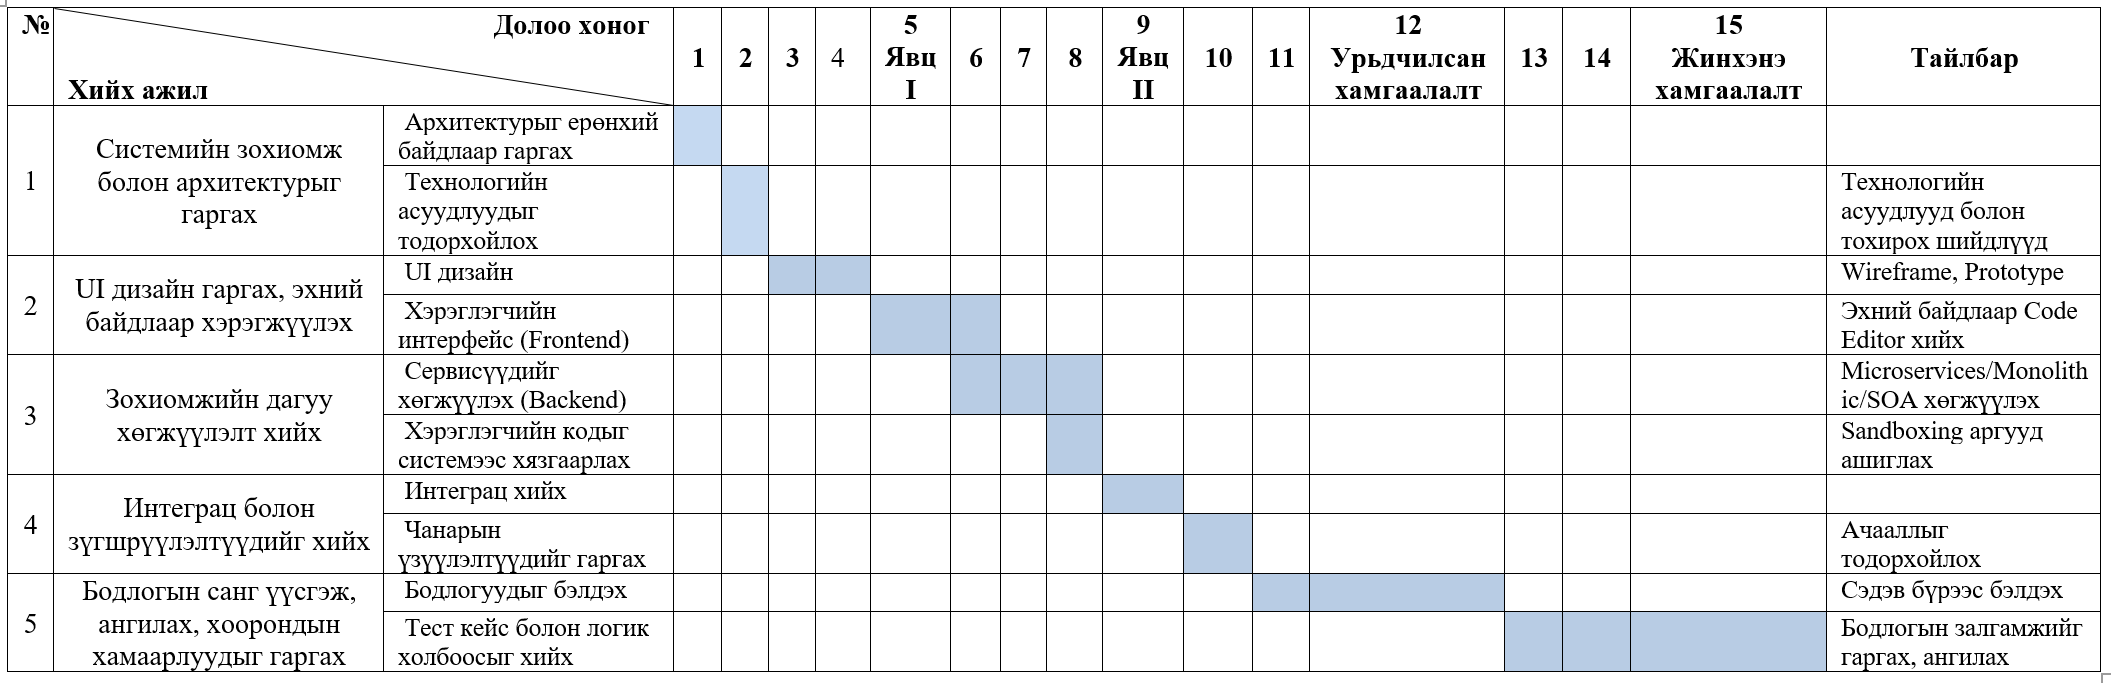
\includegraphics[angle=90, width=-10cm, height=-24cm]{img/thesis-plan.PNG}
%   \caption{Үечилсэн төлөвлөгөө}
% \end{figure}